\documentclass[fullpage,fleqn,leqno]{article}
\usepackage{../../tex/html}
\usepackage{fullpage}
%\usepackage{enumitem}
\usepackage{amsfonts,amsmath,color,amsthm,amssymb, enumerate, bbm, subfig,hyperref}

%\usepackage[normalem]{ulem}
\usepackage{graphicx}
\newcommand{\vs}[1]{\vspace{#1 pt}}

\usepackage{graphicx,amsmath,gentium,tikz,caption}
\usetikzlibrary{patterns}
\usetikzlibrary{matrix,arrows,positioning,shapes}
\usetikzlibrary{arrows.meta}
\tikzset{
  a/.style={-{Stealth[scale=1.3,angle'=45]},semithick}
}
%\usepackage{xfrac,fontspec,unicode-math}
%\setmathfont[version=cambria]{Cambria Math}
%\mathversion{cambria}
\usepackage[letterpaper, portrait, margin=1.1in]{geometry}
\usepackage{amsmath,amsthm}
\usepackage{mathtools}
\newtheorem*{definition}{Definition}
\usepackage{tcolorbox}
\tcbset{colback=white,colframe=black}
\everymath{\displaystyle}

\makeatletter
\@ifundefined{namelength}{
\newlength{\namelength}
\settowidth{\namelength}{{\bf \Large Name: }}
\newlength{\namelinelength}
\setlength{\namelinelength}{\textwidth}
\addtolength{\namelinelength}{-\namelength}
}{}

\@ifundefined{vs}{
\newcommand*{\vs}[1]{\par
  \vspace*{#1\baselineskip}%
  \@afterindentfalse
  \@afterheading
}
}{}
\makeatother



\def\fancytitle#1#2#3{
      \centerline{\framebox{\framebox{ \parbox{.8\textwidth}{ \bf ENGRI 1101 \hfill
      Engineering Applications of OR \ \ \ \  Fall 2020 \hfill #3 #1 \\
\mbox{ }\hfill
      \hfill\mbox{ } \\[1mm] \mbox{ } \hfill{\Large \bf #2}\hfill
      \mbox{ }} }}}
      
\vs 2
}

\def\handout#1#2{\fancytitle{#1}{#2}{Handout}}
\def\review#1#2{\fancytitle{#1}{#2}{Review}}
\def\homework#1#2{\fancytitle{#1}{#2}{Homework}}
\def\exercises#1{\fancytitle{}{#1}{Exercises}}
\def\solution#1#2{\fancytitle{#1}{#2}{Solutions}}
\def\final#1#2{\fancytitle{#1}{#2}{Final}
      \noindent {\bf \Large Name:} \rule{\namelinelength}{0.5pt}
      \vspace*{\baselineskip}}
\def\prelim#1#2{\fancytitle{#1}{#2}{Prelim}
      \noindent {\bf \Large Name:} \rule{\namelinelength}{0.5pt}
      \vspace*{\baselineskip}}
\def\quiz#1#2{\fancytitle{#1}{#2}{Quiz}
      \noindent {\bf \Large Name:} \rule{\namelinelength}{0.5pt}
      \vspace*{\baselineskip}}
\def\lab#1#2{\fancytitle{#1}{#2}{Lab}
      \noindent {\bf \Large Name:} \rule{\namelinelength}{0.5pt}
      \vspace*{\baselineskip}}
\def\prelab#1#2{\fancytitle{#1}{#2}{Prelab}
      \noindent {\bf \Large Name:} \rule{\namelinelength}{0.5pt}
      \vspace*{\baselineskip}}




\definecolor{purple}{RGB}{128,0,128}
\newcommand{\com}[1]{{\bf {\color{red} #1}}}

\begin{document}

\lab{3}{The Minimum Spanning Tree Problem}

\noindent
\textbf{Objectives:}
\begin{itemize}
\item Introduce students to the graph theoretic concept of spanning
  trees.
\item Show three different combinatorial algorithms for solving the
  minimum spanning tree problem.
\item Demonstrate a practical use of minimum spanning trees.
\end{itemize}


\noindent 
\textbf{Optional Reading Assignment:}
\begin{itemize}
\item
Read Handout 4 on the minimum spanning tree problem.
\end{itemize}

\textbf{Brief description:} In this lab, we review some of the
applications of the minimum spanning tree problem, along with the
concept of the spanning tree in an undirected graph (and why these are
the desired solutions for the problem), some algorithms for solving
the minimal spanning tree (MST) problem, and sensitivity analysis for
this problem.



\section{An application: communication
  network design} 
  You are the engineer in charge of designing a new
high speed fiber optic Internet network between several Operations Research departments throughout the U.S.. Your objective is to design a system that
connects various campuses. However, so that
this network can be brought online quickly, we must install the fiber
optic line within existing physical infrastructure. The possible
physical cable routes between cities and the cost of installing the
fiber optic cable (in millions of dollars) are given by the data shown
on the graph in figure~\ref{fig:marked}. How do you suppose you
would go about designing such a system? Since you can only use the
edges shown in the attached graph, you must choose a subgraph of the
given graph, or in other words, a subset of the possible edges. Every
location must be serviced which means that the subgraph must be
spanning. You should be able to get to any location from any other
location. This means the subgraph should be connected. Because you are
trying to minimize cost, the subgraph should also be minimal, meaning
that you cannot remove any of the edges while maintaining the other
necessary properties. A minimal connected spanning subgraph is called
a spanning tree. There are many other ways of defining trees. In
operations research terminology, we want to find a minimum spanning
tree of the given graph.  \\

An example of a spanning tree is indicated using thick edges in
figure~\ref{fig:marked}. Do you think that this is the best possible?  Can you briefly give a convincing argument why or why not?


\begin{figure}[htp]
  \centering

  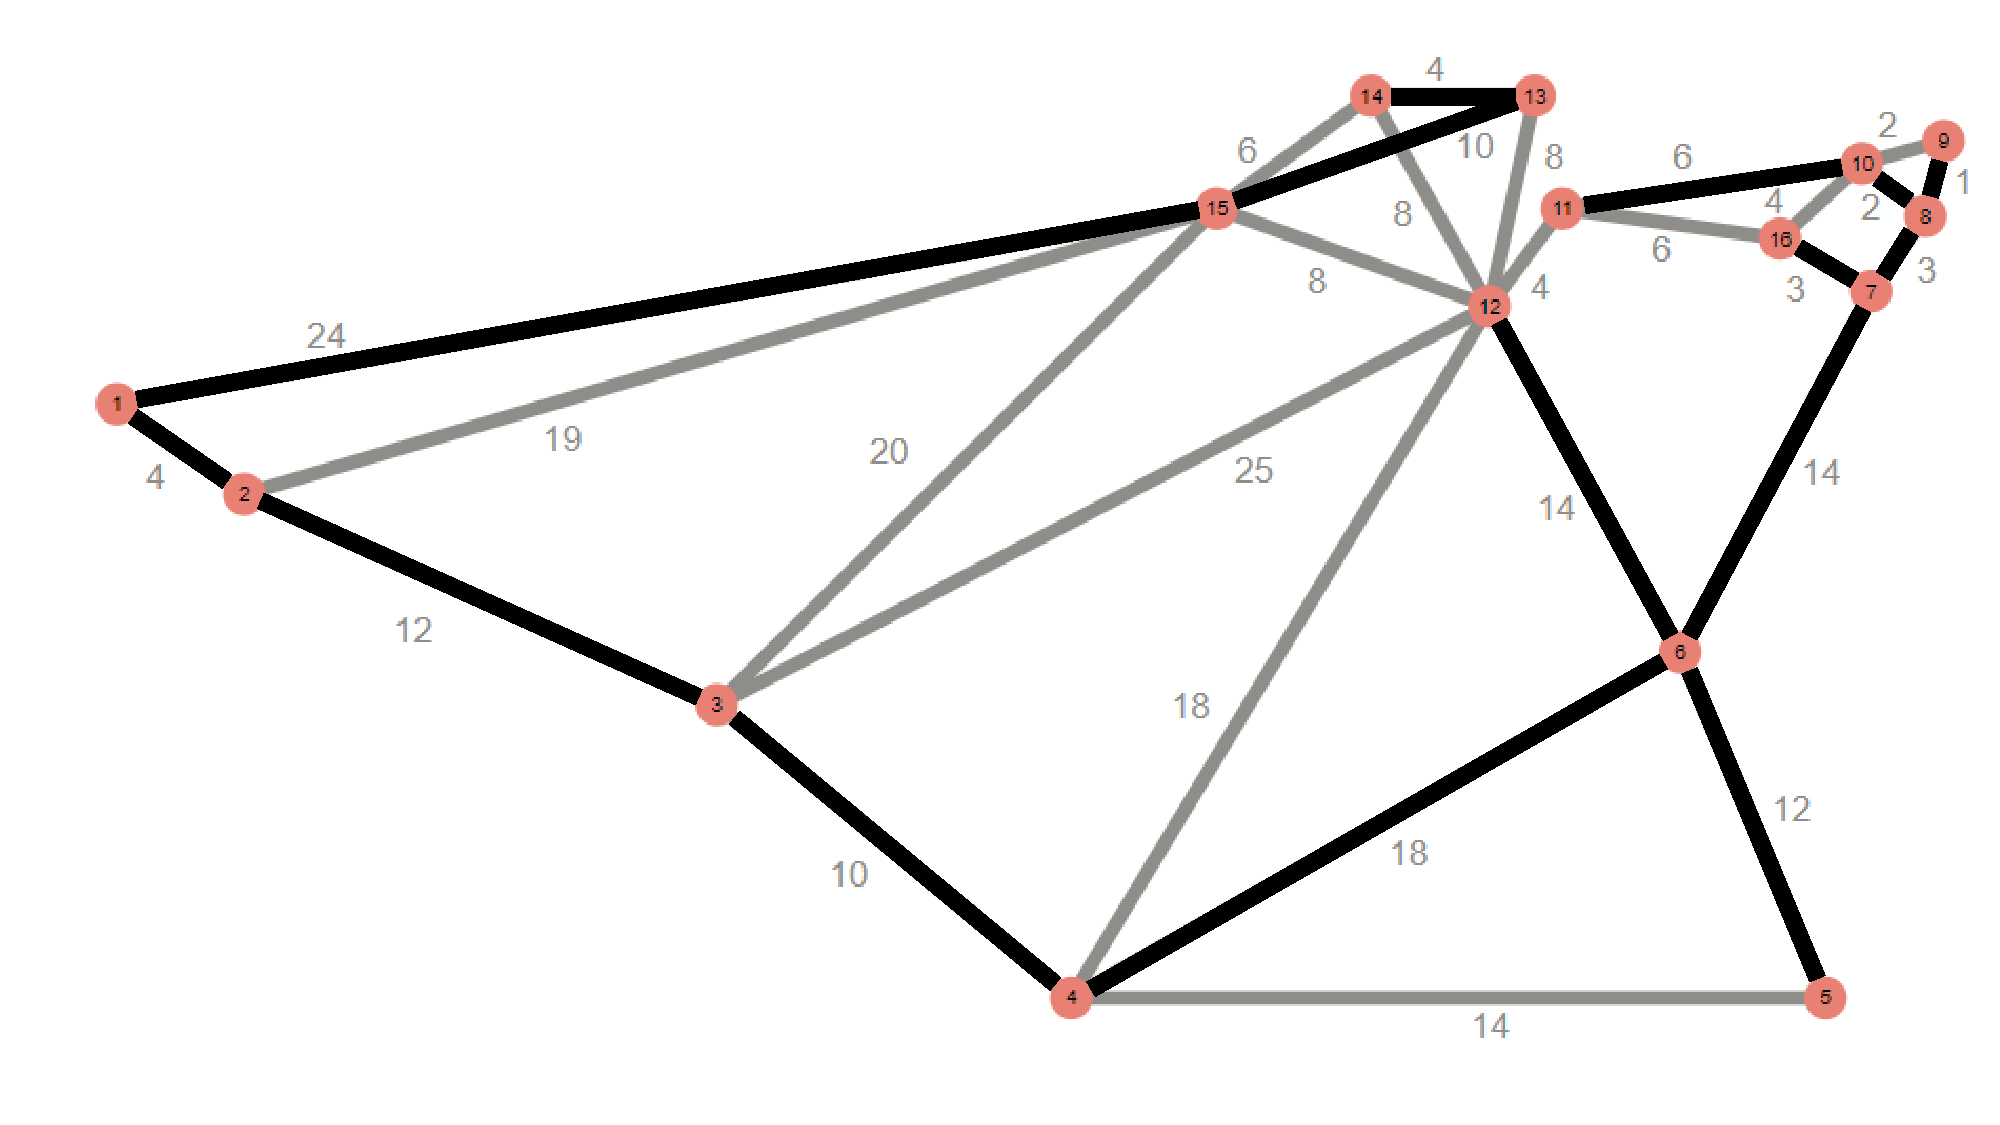
\includegraphics[width=\textwidth]{SampleTree.pdf}
  
  \caption{A spanning tree of the communications network.}
  \label{fig:marked}
\end{figure}


\newpage
\section{Minimum spanning tree algorithms}

In this section we will investigate three different algorithms for
solving the Minimum Spanning Tree Problem. 


First you will try the algorithm that you have seen on lecture: Prim's
algorithm. This algorithm works as follows:
\begin{enumerate}
\item Choose any node from which to begin, say node 1, and start the tree
with the cheapest edge from node 1 to one of the other nodes in the
graph.
\item At each subsequent step, add the cheapest edge that maintains
connectivity of the current tree and adds a new node. In other words,
add the cheapest edge that connects a new node to those already
connected.
\item Continue to do this until all nodes are connected.
\end{enumerate}

Run the first 5 iterations of this algorithm on the map below by hand. Show your work: indicate the order in which you
add the edges (e.g. by clearly writing 1 next to the first edge you added, 2 next to the second edge you added, etc).

\vspace*{3\baselineskip}

\begin{center}
  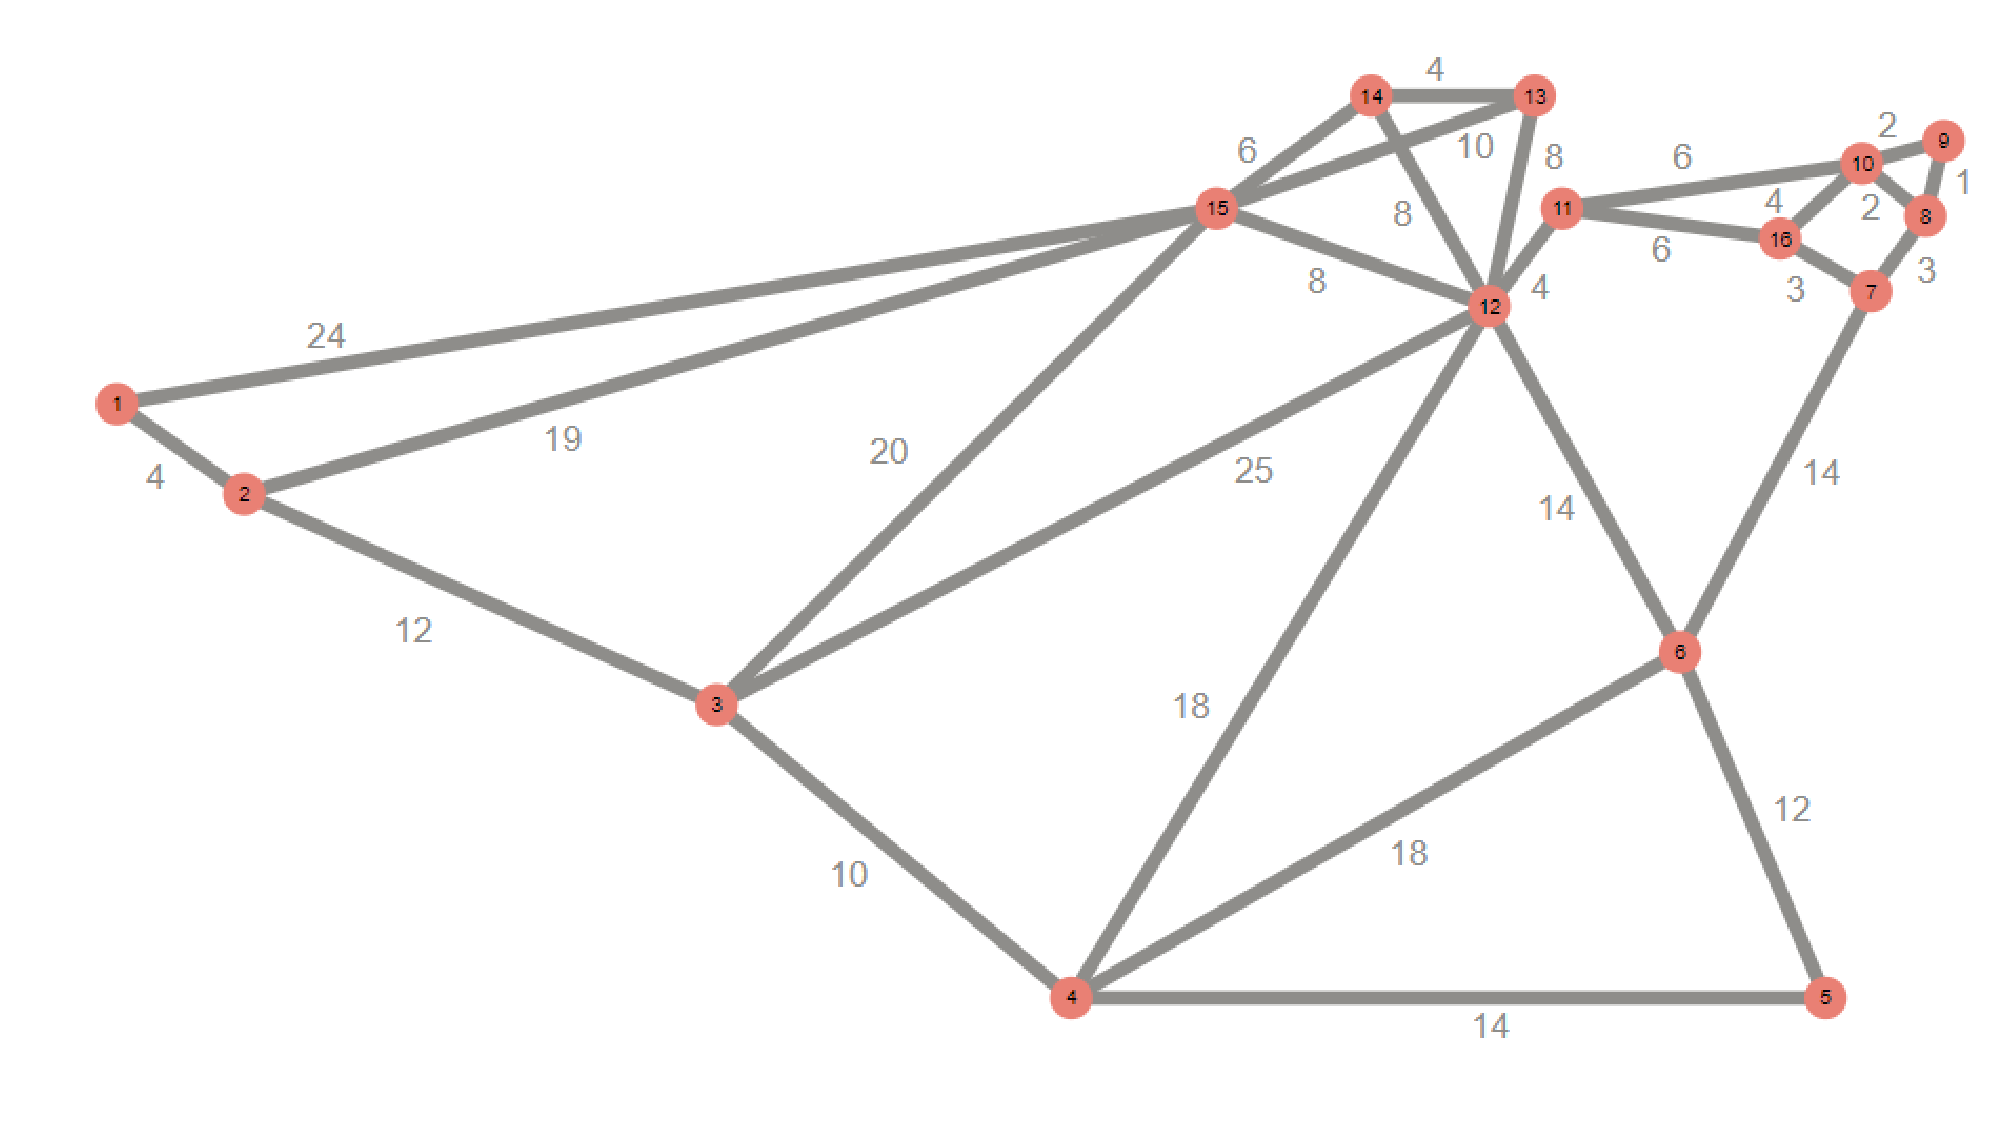
\includegraphics[width=.9\textwidth]{EmptyMST.pdf}
\end{center}

\vspace*{3\baselineskip}
\newpage
We will now let the computer help us.  To get set up, do the following:
\begin{itemize}
 \item Go to \url{http://engri1101.orie.cornell.edu/} on a web browser. 

\item Click on \texttt{Minnimum Spanning Tree}.
\end{itemize}

\vspace*{\baselineskip}

Now use the software to run the first 5 iterations of Prim's

\begin{itemize}
\item Click \texttt{Prim's} within the list of commands at the bottom of the screen (it should already be clicked for you!).
\item Click the node labeled number 1 to start running Prim's from node 1.  Node number 1 should turn blue, and you will be prompted ``Click the first edge to start.''
\item Click the first edge you labeled while starting Prim's by hand.  If that was the correct first edge to add, the edge will darken.  If it was not the correct edge to add, it will flash red and allow you to try again.
\item Repeat this process, iteratively the first five edges of the minimum spanning tree.
\end{itemize}

Did you make any mistakes during your first five iterations?

\vspace*{6\baselineskip}

The program uses colors to distinguish different types of
information. Using your observations about the first 5 iterations,
explain when each of the following represents.

\begin{itemize}
\item red nodes
\item blue nodes
\end{itemize}
\vspace*{4\baselineskip}


Hit the \texttt{Hint} button at the bottom of the graph.  Several edges will flash light blue, and in the next iteration you will add one of these edges. Which of the highlighted edges should you add next?  

\vspace*{4\baselineskip}

What characterizes which edges the program flashes?  For example, which edge(s) would the \texttt{Hint} feature have flashed after you had only added the first edge?  Feel free to restart the program and check your work.

\clearpage

Now continue with the program until it completes the computation of a
minimum spanning tree.  Add the edges one at a time, predicting what the algorithm will do in its next step. What is the total
cost of this tree, and how does this compare with the original tree?


\vspace*{6\baselineskip}

Now we turn to another algorithm which is called Kruskal's
Algorithm. This is an example of a so- called Greedy Algorithm,
i.e. an algorithm that always takes the step that ``looks best''
currently. Greedy algorithms are widely used in computer science
beyond just solving the MST. Kruskal's algorithm works as follows:

\begin{enumerate}
\item Begin with the cheapest edge (break ties arbitrarily).
\item At each step, add the cheapest edge not already in the system that
does not create a cycle, or a loop in the system.
\item Continue adding edges until you get a spanning tree.
\end{enumerate}

Run the first 5 iterations of this algorithm by hand on the map below.
\vspace*{3\baselineskip}

\begin{center}
  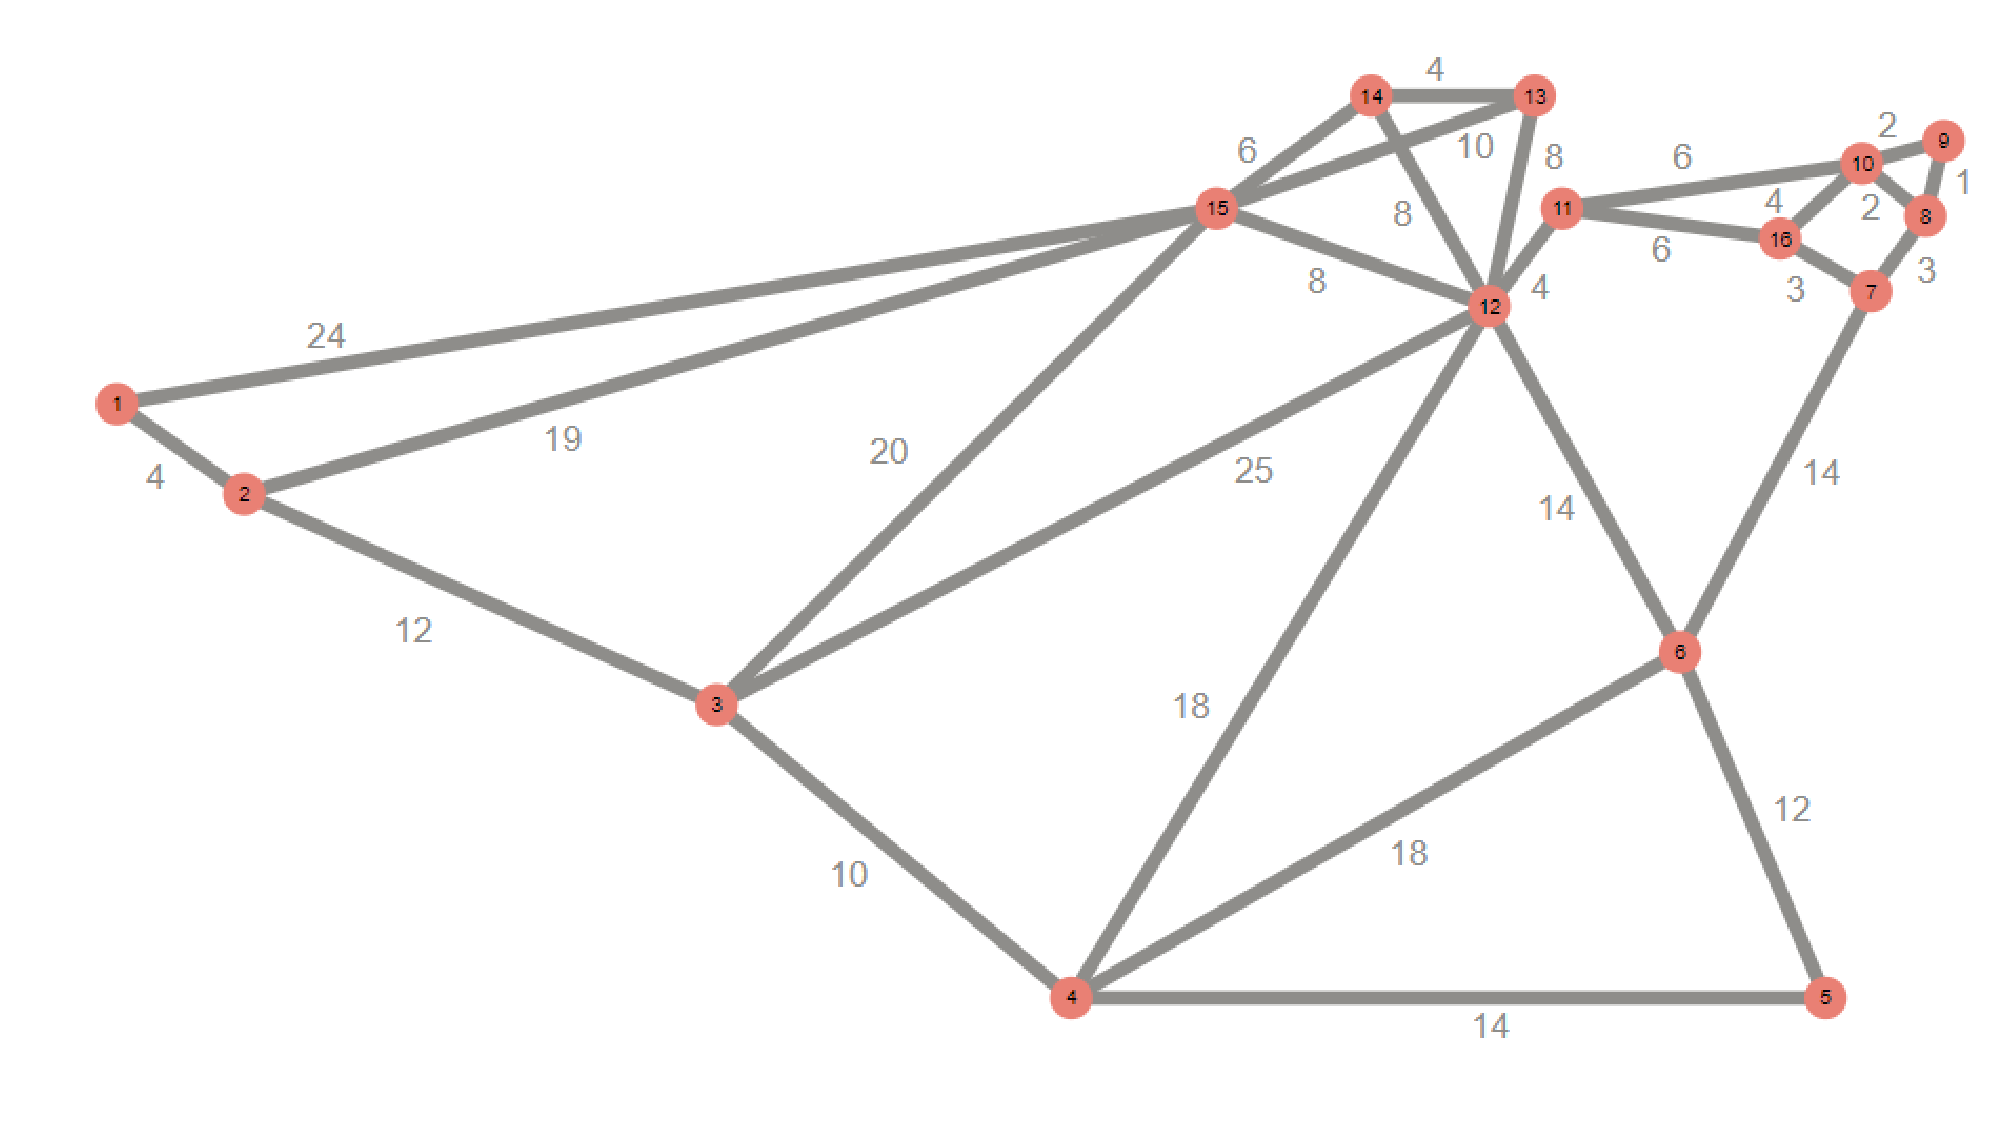
\includegraphics[width=.9\textwidth]{EmptyMST.pdf}
\end{center}

\vspace*{3\baselineskip}

Indicate edges that you have decided to include on the above blank
copy of the map, and also indicate (differently) any edges of these
that you you considered adding (but decided not to because they created a cycle or loop). Again, specify the order in
which you are adding the edges.

\vspace*{\baselineskip}


\newpage

Now you will trace a complete execution of Kruskal's algorithm on this
data. You can start Kruskal's algorithm by clicking \texttt{Kruskal's} on the bottom of the page, and then following prompts: click the edges to add them in order.

First start by comparing the first 5 iterations of the
computer's run with your first 5 iterations. Did you make any mistakes?



\vspace*{6\baselineskip}

Now continue running the algorithm until it finishes. As before, try to anticipate each of the algorithm's
steps. What is the cost of the final solution? 

\vspace*{5\baselineskip}
Is the same spanning
tree found by the two algorithms? 

\vspace*{6\baselineskip}
(Why is the previous question not a
dumb question?)

\vspace*{6\baselineskip}

\newpage

The following algorithm is called the Reverse Greedy Algorithm, and it
effectively does Kruskal's in reverse.

\begin{enumerate}
\item Start with the entire graph.
\item At each step, check if the graph has a cycle. If it does, remove
the most expensive edge in the cycle (break ties arbitrarily, and pick any cycle you'd like).
\item Continue to do this until the graph remaining is a spanning tree.
\end{enumerate}
\vspace*{1\baselineskip}

Try the algorithm by hand on this last blank copy of the map.  Do the first five iterations by hand.  Then use the software to check your work:  Start Reverse Kruskal's by clicking \texttt{R-Kruskal's} and then hit Fast-Forward, watching the software remove edges one at a time.  Note: this software works a little bit different than the above process, and it always looks for the most expensive edge it can eliminate.  It will run a version of Reverse Kruskal's, but won't run in the full generality as above.

\vspace*{1.5\baselineskip}

\begin{center}
  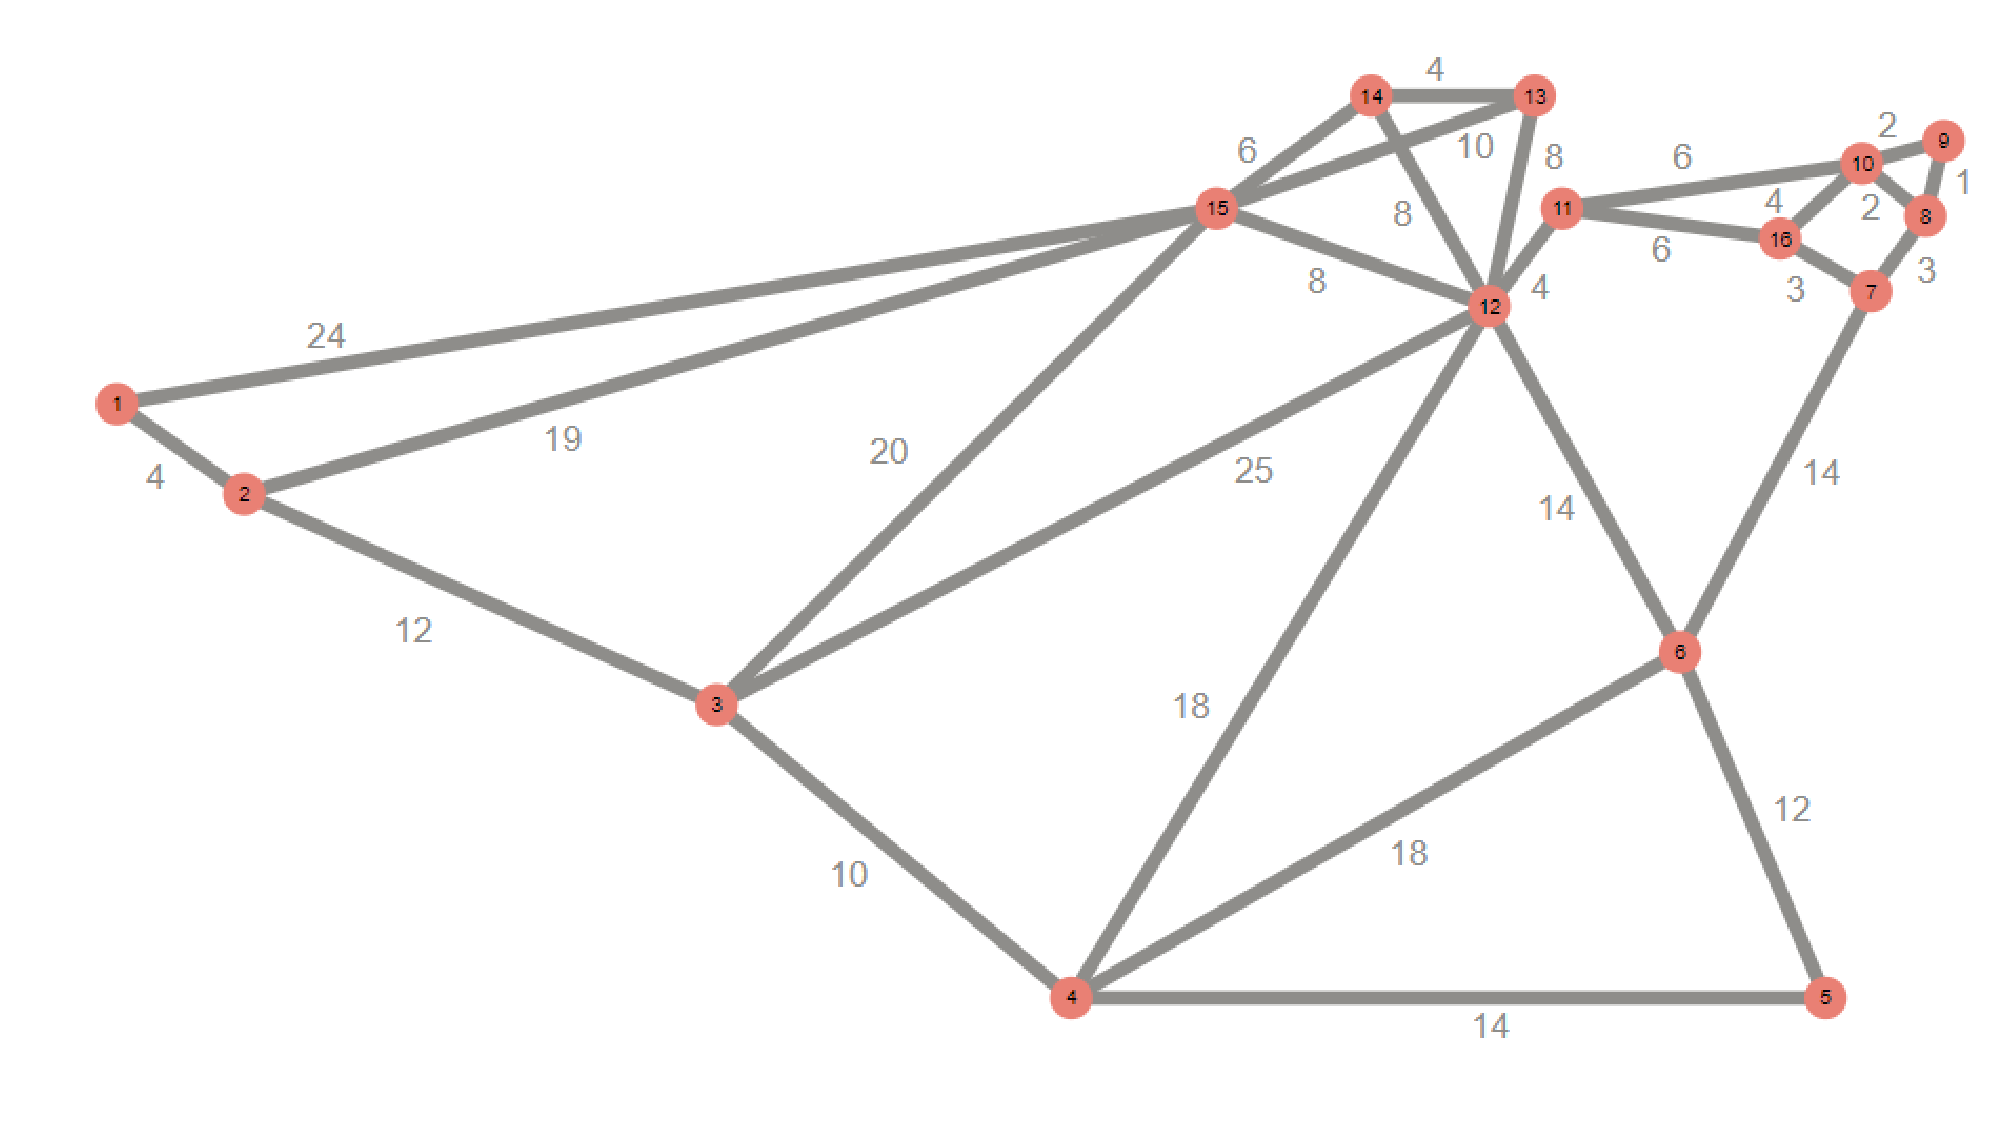
\includegraphics[width=.9\textwidth]{EmptyMST.pdf}
\end{center}

\vspace*{\baselineskip}

What is
the cost of the resulting spanning tree? 

\vspace*{3\baselineskip}

How does the spanning tree
and its cost compare to those obtained by the previous algorithms?

\vspace*{3\baselineskip}

Which of the three algorithms was the easiest for you to follow? Why?

\vspace*{3\baselineskip}

\section{Analyzing minimum spanning trees}

Suppose you start with some spanning tree, like the first one given in
your lab handout, can you devise a way to systematically improve it? In
other words, given a spanning tree, can you tell if it is one of
minimum cost and, if not, can you improve it (without recomputing a
minimum spanning tree from scratch)? Suggest such an algorithm.


\vspace*{6\baselineskip}


Next we will study how the solution changes when problem parameters
are altered. This is referred to as Sensitivity Analysis. Consider
edge $\{4, 6\}$ which was not used in the minimum spanning tree found
by Prim's algorithm. Just this one edge's cost will be changed. Should
it increase or decrease if it will be included in the new minimum
spanning tree? Exactly what must the cost of $\{4, 6\}$ be changed to
for this to occur?  

\vspace*{6\baselineskip}

Check your work using the software: 
\begin{itemize}
\item Click \texttt{Sensitivity}
\item Enter node number 4 into the prompt and hit OK
\item Enter node number 6 into the prompt and hit OK
\item Enter 1  less than the cost you answered above\footnote{For example, if you answered that the cost must be 7 for it to be included in the new MST, you'd enter 6 at this step.} and hit OK.
\item Click \texttt{Prim's}, click node 1, and then click \texttt{Fast Forward} to quickly rerun Prim's with the new edge length
\end{itemize}
Is the edge $\{4, 6\}$ now in the tree?  Follow the above process and reset the length of the edge $\{4, 6\}$ to be 2 more than it currently is\footnote{E.g. if you just reset the cost of edge $\{4, 6\}$ to be 6, you'd now set it to be 8 -- one more than you answered above} and re-run Prim's from node 1.  Is the edge $\{4, 6\}$ no longer in the tree?

\vspace*{6\baselineskip}


In general, what does this suggest about how the cost of any one ``not
included'' edge must be changed if it is to be included in the minimum
spanning tree for the modified data?

\vspace*{8\baselineskip}


Now consider an edge that is in the minimum spanning tree, such as
$\{1, 2\}$. How must this be changed for this edge in order for this
edge to be forced out of the optimal solution? Again, also figure out
the general rule for forcing minimum spanning tree edges out of the
minimum spanning tree.

  

\end{document}